\documentclass[landscape]{foils} 
\input{../common-preamble-start}
\input{../preamble.tex}

\usepackage{url}
\usepackage{hyperref}
\hypersetup{backref,  pdfpagemode=FullScreen,  linkcolor=blue, citecolor=red, colorlinks=true, hyperindex=true}


\usetikzlibrary{trees,arrows,positioning}

\tikzset{stream/.style={rectangle,rounded corners,draw= red!50,fill=white,thick,minimum width=6cm,minimum height=3cm}}
\tikzset{hidden/.style={rectangle,draw=white,fill=white,thick}}
\tikzset{analysis/.style={rectangle,rounded corners,draw=black!50,fill=white,thick,minimum width=6cm,minimum height=10cm}}
\tikzset{charmatrix/.style={rectangle,draw=none,fill=black,minimum width=6cm,minimum height=8mm}}
\tikzset{augmat/.style={rectangle,draw=none,fill=red,minimum width=6cm,minimum height=15mm}}
\tikzset{tree/.style={rectangle,draw=black,fill=black,minimum width=6cm,minimum height=8mm}}
\tikzset{inf/.style={rectangle,rounded corners,draw=black!50,fill=green!20,thick,minimum width=6cm,minimum height=2cm}}
\tikzset{toArrow/.style={stealth-,ultra thick}}


\begin{document}
\pagecolor{white}

\myNewSlide
\section*{What happened? (more or less)}
\begin{compactitem}
	\item I clicked on the Terminal.app icon in the Dock
	\item Some device driver noted that a click had occurred.
	\item The OS noticed
	\item The OS checked where the cursor was
	\item The OS did some calculations and determined that it was in the ``Dock''
	\item The OS told the \path{Dock} process that a click had occurred.
	\item By asking the OS and doing calculations, the \path{Dock} determined that it was the Terminal.app icon that was clicked.
	\item The \path{Dock} process told the OS to tell the \path{Finder} to launch Terminal.app
	\item \path{Terminal} was launched and {\color{green} it negotiated with the OS and \path{WindowServer} to display a window.}
	\item {\color{green} The \path{Terminal} launched a process called \path{login}}
	\item {\color{black} \path{login} read a history file. Based on this information it wrote a message to its standard output stream. }
	\item {\color{green} \path{Terminal} is reading \path{login}'s output, and \path{Terminal} makes the window display the message.}
	\item {\color{black} \path{login} launched a process called \path{bash}}
	\item {\color{red} \path{bash} initialized itself (by reading files such as\\ \path{/Users/mholder/.bash\_profile})}
	\item {\color{red}\path{bash} wrote its prompt (the characters `$\sim$ 500 \$ ') to its standard error stream.}
	\item {\color{green}\path{Terminal} has wrapped up bash's standard streams (input, output and error stream). When
	it detects that bash wrote something \path{Terminal} does some OS calls to draw the characters in the window.}
	\item {\color{red}\path{bash} told the OS through some function we'll call ``readNextLineOfInput'' that it wanted to read the next line from standard input.  Because there was no input, the execution of the \path{bash}'s process hangs.}
	\item I typed `l'
	\begin{compactenum}	
		\item a keyboard device drive noticed the key was hit and told the OS
		\item the OS asked the window manager what application had ``focus'' -- the answer was \path{Terminal}
		\item The OS told the \path{Terminal} that there was a key-down event
		\item {\color{green}The \path{Terminal} (with help of OS)  the letter `l'}
		\item {\color{green}The \path{Terminal} wrote `l' to a stream that (via OS functions) was connected to \path{bash} standard input}
		\item {\color{green}The \path{Terminal} displayed the letter `l' in the Window}
		\item {\color{red}Because it was not a carriage return, the `readNextLineOfInput' function stored the character, but did not return anything to \path{bash}. So \path{bash} still has not heard anything yet.}
	\end{compactenum}
	\item I typed `s' -- same steps as for when I typed `l'
	\item I typed the `return' key -- steps 1-6 occurred as before.
	\item {\color{red}The `readNextLineOfInput' function that \path{bash} called returned the string `ls$<$newline$>$'}
	\item {\color{red}\path{bash} (through rules we'll talk about later) determined that `ls' means that I wanted to run the program called \path{ls} with no command line arguments.}
	\item Via negotiations with the OS, {\color{red}\path{bash} launched \path{ls}}
	\item Any standard input of \path{bash} will now be redirected to \path{ls}, and the standard output of \path{ls} will be written to the stream, but it will be redirected to \path{bash}'s stdandard output.
	\item \path{ls} checked to see if it got any command line arguments (it did not).
	\item \path{ls} asked the OS what it should use as its working directory (The OS said '/Users/mholder').
	\item \path{ls} asked the OS for the contents of the file '/Users/mholder'
	\item The OS dealt with some filesystem device driver software to get the contents and return the answer.
	\item \path{ls} filtered out any entries in that file that started `.'
	\item \path{ls} queried the OS to find out how many characters wide its standard output was.
	\item \path{ls} formatted the entries such that they fit nicely in the width.
	\item \path{ls} wrote the formatted strings to its standard output.
	\item {\color{red}That standard out from \path{ls} is passed to \path{bash}'s standard output}
	\item {\color{green}\path{Terminal} is reading \path{bash}'s output, and it makes sure that the output is displayed in the window that we see.}
	\item The \path{ls} process is exits
	\item {\color{red}\path{bash} detects that \path{ls} exited. It writes it's prompt again.}
	\item {\color{green}\path{Terminal} displays the latest output from \path{bash}, which is the new prompt.}	
		
\end{compactitem}


\myNewSlide
\path{ls} never deals with \path{bash} (and certainly not with processes further up stream such as \path{login} or \path{Terminal}).
\path{ls} just:
\begin{compactitem}	
	\item checks its command-line arguments,
	\item asks the the operating system some context information,
	\item composes an answer to its assigned task,
	\item writes the answer to its standard output stream,
	\item exits
\end{compactitem}

\myNewSlide
\path{bash} never deals with \path{login} or \path{Terminal}.  It just:
\begin{compactenum}	
	\item checks its command-line arguments,
	\item asks the the operating system some context information,
	 \item reads a line of input from standard input,
	\item takes the action requested,
	\item writes ``the answer'' to through its output and error streams,
	\item goes back to step 3
\end{compactenum}

\path{bash} is a shell that is often used to launch other processes. 
So the ``action'' in step 4 is often: ``launch a process and redirect your streams to the new process until it exits.''


\myNewSlide
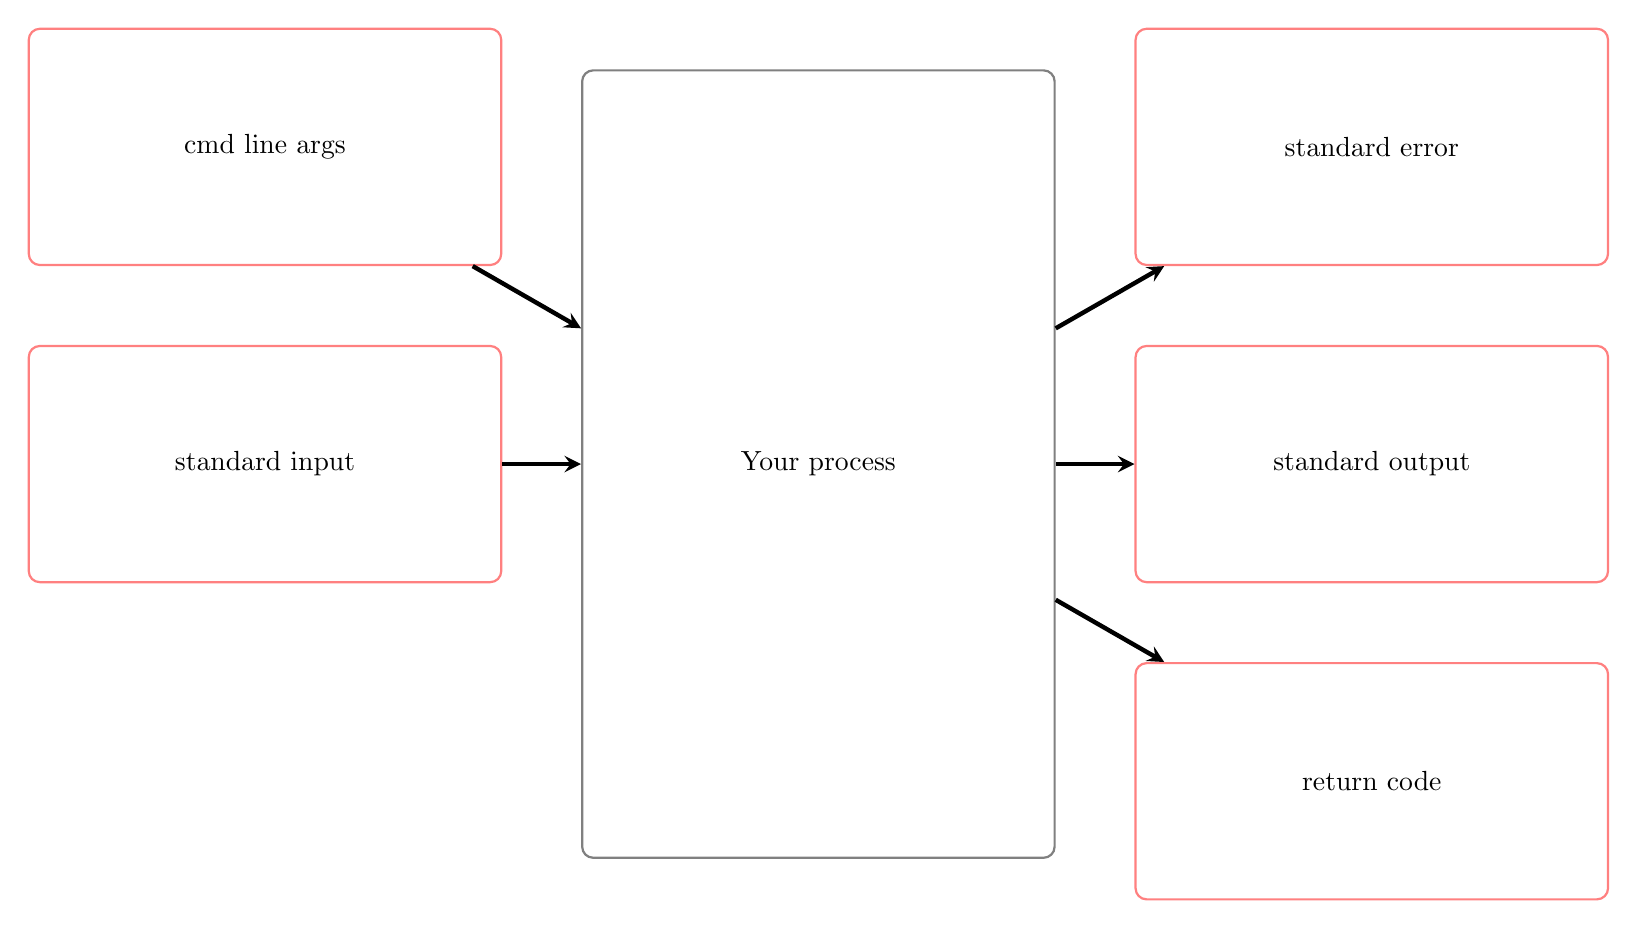
\begin{tikzpicture}
\begin{scope}[node distance=10mm]
	\node (args) [stream] {cmd line args} ;
	\node (stdin) [stream, below =of args] {standard input} ;
	\node (proc)  [analysis, right =of stdin] {Your process} edge [toArrow] (args)  edge [toArrow] (stdin);
	\node (stdout) [stream, right =of proc] {standard output} edge [toArrow] (proc);
	\node (stderr) [stream, above =of stdout] {standard error}  edge [toArrow] (proc) ;
	\node (retcode) [stream, below =of stdout] {return code}  edge [toArrow] (proc) ;
\end{scope}
\end{tikzpicture} 


\myNewSlide
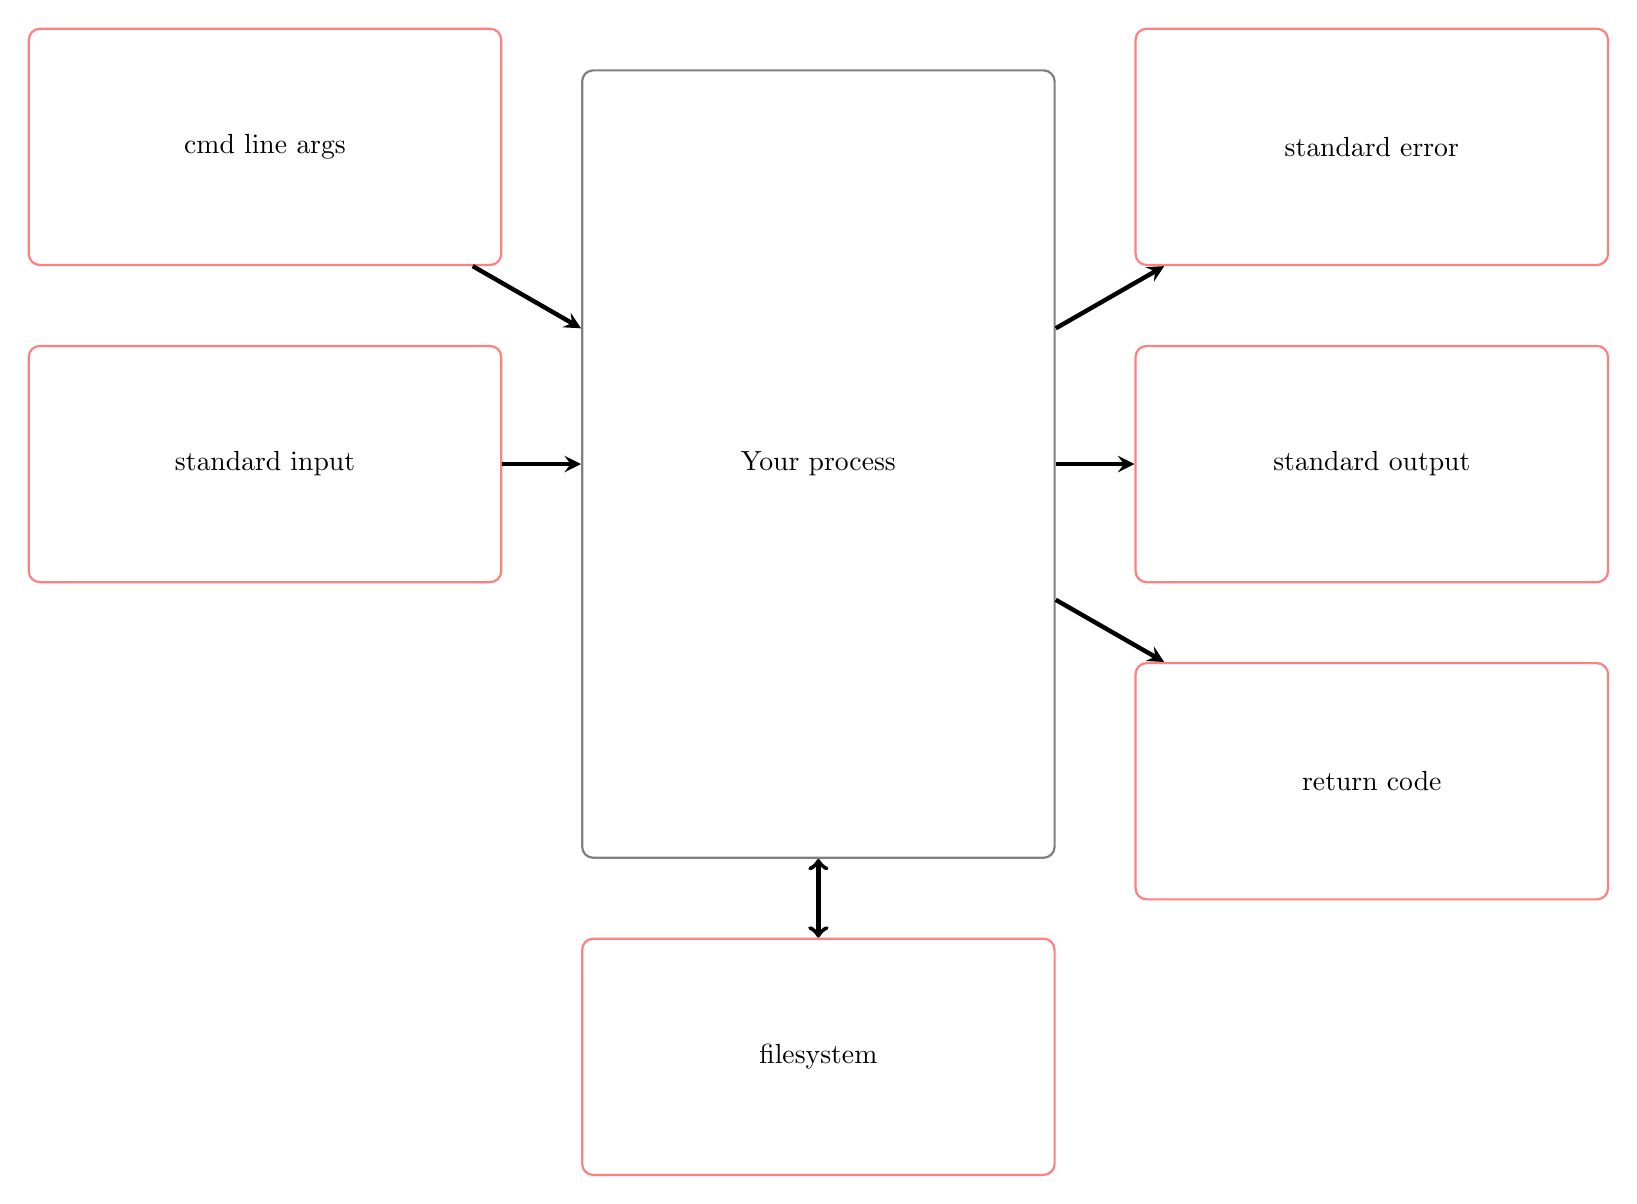
\begin{tikzpicture}
\begin{scope}[node distance=10mm]
	\node (args) [stream] {cmd line args} ;
	\node (stdin) [stream, below =of args] {standard input} ;
	\node (proc)  [analysis, right =of stdin] {Your process} edge [toArrow] (args)  edge [toArrow] (stdin)  ;
	\node (fs) [stream, below =of proc] {filesystem} edge [<->,ultra thick] (proc);
	\node (stdout) [stream, right =of proc] {standard output} edge [toArrow] (proc);
	\node (stderr) [stream, above =of stdout] {standard error}  edge [toArrow] (proc) ;
	\node (retcode) [stream, below =of stdout] {return code}  edge [toArrow] (proc) ;
\end{scope}
\end{tikzpicture} 




\myNewSlide
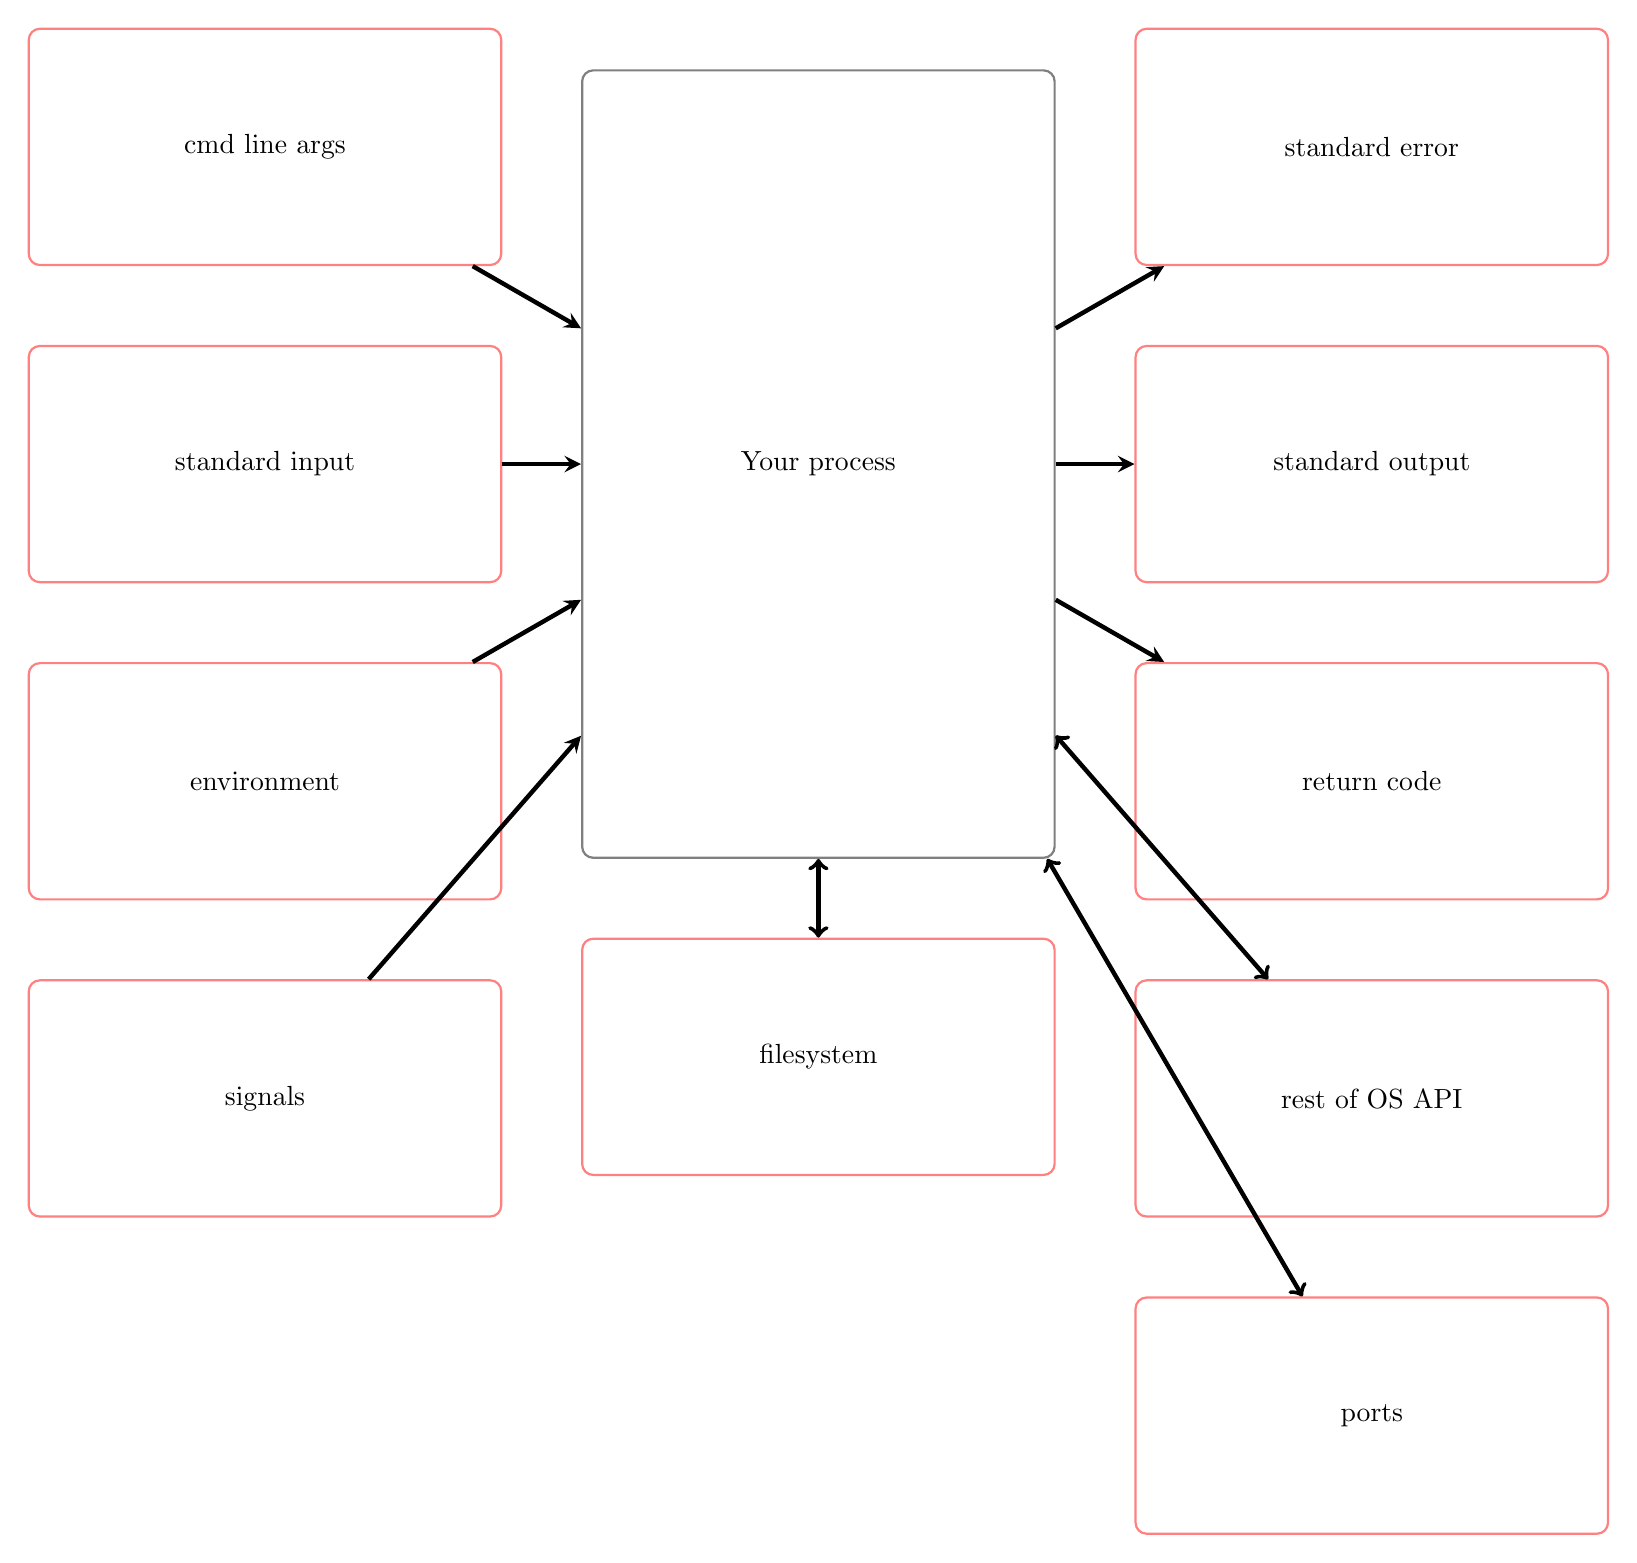
\begin{tikzpicture}
\begin{scope}[node distance=10mm]
	\node (args) [stream] {cmd line args} ;
	\node (stdin) [stream, below =of args] {standard input} ;
	\node (env) [stream, below =of stdin] {environment}  ;
	\node (signals) [stream, below =of env] {signals}  ;
	\node (proc)  [analysis, right =of stdin] {Your process} edge [toArrow] (args)  edge [toArrow] (stdin) edge [toArrow] (env) edge [toArrow] (signals);
	\node (fs) [stream, below =of proc] {filesystem} edge [<->,ultra thick] (proc);
	\node (stdout) [stream, right =of proc] {standard output} edge [toArrow] (proc);
	\node (stderr) [stream, above =of stdout] {standard error}  edge [toArrow] (proc) ;
	\node (retcode) [stream, below =of stdout] {return code}  edge [toArrow] (proc) ;
	\node (sys) [stream, below =of retcode] {rest of OS API} edge [<->,ultra thick] (proc);
	\node (port) [stream, below =of sys] {ports} edge [<->,ultra thick] (proc);
\end{scope}
\end{tikzpicture} 


\myNewSlide
\section*{Shells}
The interface to the OS and kernel is a huge number of functions -- it easy to invoke these functions in the wrong way, and their ``raw'' response is often cryptic.

Shells:
\begin{compactenum}	
	\item protect the kernel  -- rather than pounding the kernel with our typos, the shell composes valid requests.
	\item make the raw output of system functions human-readable.
\end{compactenum}	

The kernel does not understand text like `ls'

Shells are simple programming language interpreters that take text that humans write, and convert it into instructions for the machine.
\myNewSlide
\section*{Compiled versus interpreted programming languages}
\large
Compiled languages:\\
1. {\color{red} Your program} $\rightarrow$ (compiler) $\rightarrow$ executable\par
Then you have to launch the executable:\\
2. executable $\rightarrow$ (kernel) $\rightarrow$ running process $\rightarrow$ {\color{red} Your results}\\

Interpreted languages:\\
1. interpreter executable $\rightarrow$ (kernel) $\rightarrow$ running interpreter process\\
2. {\color{red} Your script}  $\rightarrow$ (interpreter process) $\rightarrow$ {\color{red} Your results}

\end{document}
